

\begin{figure}
\begin{mdframed}[backgroundcolor=gray!04] 
\begin{scriptsize}

{\large \textbf{Task: NY Times}} \bigskip


New York Times has an archive with all its articles published articles at a given date. An example of the articles is shown below

\medskip

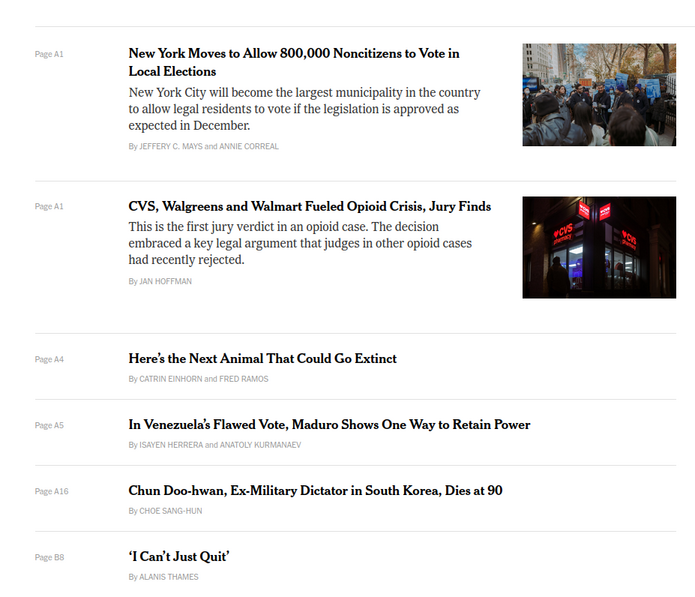
\includegraphics[width=\textwidth]{appendix/cp6/rsz_nytimes.png}

\medskip

\begin{center}
\rule{10cm}{0.4pt}
\end{center}

\textbf{Task} \medskip



Given a \code{string} representing the url for NY Times Today's, you must write a Python script using the \code{BeautifulSoup} and \code{requests} modules to scrap all the headlines of that page. \medskip



Details:\medskip


Web scrapping relies on the HTML elements of the page. You can find more information by:

\begin{enumerate}


    \item  Right-clicking a page in your web browser

    \item  Selecting \code{view page source}


\end{enumerate}

\end{scriptsize}
\end{mdframed}
\end{figure}
  


\begin{figure}
\begin{mdframed}[backgroundcolor=gray!04] 
\begin{scriptsize}



\textbf{Input} 


\begin{python}
url = "https://www.nytimes.com/issue/todayspaper/" \
  "2021/11/01/todays-new-york-times"
\end{python}

\textbf{Output}


\begin{python}
result = [ 
  "Angling for a Merry Fishmas Despite Global Shipping Delays",
  "Who Had Covid-19 Vaccine Breakthrough Cases?", ...
]
\end{python}



\begin{center}
\rule{10cm}{0.4pt}
\end{center}



\textbf{Input}

\begin{python}
url = "https://www.nytimes.com/issue/todayspaper/" \
  "2021/10/01/todays-new-york-times"
\end{python}

\textbf{Output}


\begin{python}
result = [ 
  "Leader of Prestigious Yale Program Resigns, Citing Donor Pressure",
  "After Hurricane Ida, Oil Infrastructure Springs Dozens of Leaks", ... 
]
\end{python}


\textbf{Explanation} \medskip


These are some of the articles in each input web page. Since the list is quite extensive, the output provides an excerpt of the articles found in each input page. 



\begin{center}
\rule{10cm}{0.4pt}
\end{center}
  


\textbf{Resources}

\begin{itemize}
    \item \href{https://docs.python-requests.org/en/latest/}{Requests: HTTP for Humans}
    \item \href{https://docs.python-requests.org/en/latest/api/}{Requests API}
    \item \href{https://www.crummy.com/software/BeautifulSoup/bs4/doc/}{Beautiful Soup Documentation}
    \item \href{https://www.dataquest.io/blog/web-scraping-python-using-beautiful-soup/}{Tutorial: Web Scraping with Python Using Beautiful Soup}
    \item \href{https://stackoverflow.com/questions/2612548/extracting-an-attribute-value-with-beautifulsoup}{Extracting an attribute value with beautifulsoup}
    \item \href{https://stackoverflow.com/questions/6287529/how-to-find-children-of-nodes-using-beautifulsoup}{How to find children of nodes using BeautifulSoup}
    \item \href{https://stackoverflow.com/questions/5041008/how-to-find-elements-by-class}{How to find elements by class}
    \item \href{https://stackoverflow.com/questions/9029287/how-to-extract-http-response-body-from-a-python-requests-call}{How to extract HTTP response body from a Python requests call?} 
    \item \href{https://realpython.com/beautiful-soup-web-scraper-python/}{Beautiful Soup: Build a Web Scraper With Python}
    \item \href{https://www.scrapingbee.com/blog/python-web-scraping-beautiful-soup/}{Web Scraping with BeautifulSoup}
\end{itemize}

\end{scriptsize}
\end{mdframed}
\caption{Description for the NYTimes task}
\end{figure}

    